\section{Constructing the Concrete Implementation}
\label{04_02}

With the abstract syntax in place, the concrete syntax is the next step. The goal here, is to give each function from the abstract syntax a proper linearization so it can understand linear logic. We will need two concrete implementations in total. One for reading and understanding the Celf syntax for linear logic (like the example at the end of section \ref{03_01_03}), and one for understanding English.

\subsection{Concrete linear logic implementation}
\label{04_02_01}

The first concrete implementation we will look at is the one for understanding linear logic, as it is the most important one. Without it, we will not be able to parse the formulas and therefore will not be able to translate them into other languages. Where the abstract syntax was explained starting with the positive and negative types, the concrete syntax will be explained starting with the arguments.

\lstCode{The linearization of the \cf{Arg}uments.}{04_02_C06}
\begin{lstgf}
        -- Arguments
        _Arg A a                        = ss ( a.s ) ;
        _ArgNil                         = ss ( "nil" ) ;
        _ArgZ                           = ss ( "z" ) ;
        _Arg1                           = ss ( "1" ) ;
        _ArgMinus a                     = ss ( "( s !" ++ a.s ++ ")" ) ;
        _ArgPlus a                      = ss ( "( p !" ++ a.s ++ ")" ) ;
        _ArgList a b                    = ss ( "( cons !" ++ a.s ++ "!" ++ b.s ++ ")" ) ;
        _ArgEmptyList                   = ss ( "[]" ) ;
\end{lstgf}

Remember that \cf{\_Arg} is the function that handles the bound variables. While it takes both\cf{ ArgType} as argument (\cf{A}), it is not used. With the type of the argument already given in the universal quantification, there is no need to the type of the argument next to the argument itself. \cf{\_Arg} therefore only returns the bound variable, which makes it easier for everything else to work with it.

The rest of the \cf{Arg}s are self-explanatory. \cf{\_ArgNil}, \cf{\_ArgZ} and \cf{\_Arg1} simply look for the value they represent. Again, they are arguments that can be used in any logical formula, and are therefore hardcoded into the program. Their values will never change, no matter what formulas are being worked with. \cf{\_ArgPlus}, \cf{\_ArgMinus }and \cf{\_ArgList} have been written to use Celf's syntax (see section 3.1.2) and should look familiar.

Next after the arguments, \cf{Math} and \cf{Ident} are the simplest. As they take up a lot of room, we will look at them individually, starting with \cf{Math}.

\lstCode{The linearization of \cf{Math}}{04_02_C07}
\begin{lstgf}
        -- Mathematic operations
        _MathArg arg1                   = ss ( arg1.s ) ;
        _FinalFormula m1 ms m2          = ss ( ms.s ++ m1.s ++ m2.s ) ;
        _MathArgs arg1 mo arg2          = ss ( "(" ++ arg1.s ++ mo.s ++ arg2.s ++ ")" ) ;

        -- Arithmetic operations
        _Division                       = ss ( "/" ) ;
        _Multiplication                 = ss ( "*" ) ;
        _Addition                       = ss ( "+" ) ;
        _Subtraction                    = ss ( "-" ) ;

        -- Inequality operations
        _Greater                        = ss ( "!nat-greater" ) ;
        _GreaterEqual                   = ss ( "!nat-greatereq" ) ;
        _Equal                          = ss ( "!nat-eq" ) ;
        _LessEqual                      = ss ( "!nat-lesseq" ) ;
        _Less                           = ss ( "!nat-less" ) ;
\end{lstgf}
The values for the \cf{ArithmeticOperation}s are their normal symbol. The \cf{InequalityOperation}s, however, use the syntax described in section \ref{03_01_03}. For example, $>$ becomes "!nat-greater".

Looking at the \cf{Math} part, it is a bit more advanced. \cf{\_Math} is simple enough. Its value is that of the \cf{Arg} is is given. \cf{\_MathArgs} is the function that takes care of arithmetic operations between arguments and is surronded by a pair of paratheses. Throughout the voting protocol formulas, this is actually not used, but we will support it anyway.

\cf{\_FinalFormula} is the formula that handles inequality operations. Looking at it, one will see that the value it returns has the inequality operation first followed by the two parameters. This is the syntax Celf uses and is thus not an error. One may also notice that the order of the parameters for \cf{\_FinalFormula} is not the same as the linearization of it. The normal way to read "x is greater than y" is "x $>$ y" and is how the abstract tree is put together (see line 7 in \refCode{04_01_C04} on page \pageref{code:04_01_C04}). The concrete implementation is allowed to choose its own way of using the parameters, and can therefore use Celf's notation easily. The formula will be parsed correctly into the abstract syntax anyway.

\lstCode{The linearization of \cf{Ident}}{04_02_C08}
\begin{lstgf}
        -- Identifiers
        Ident_Uncounted a b             = ss ( "uncounted-ballot" ++ a.s ++ b.s ) ;
        Ident_Counted a b               = ss ( "counted-ballot" ++ a.s ++ b.s ) ;
        Ident_Hopeful a b               = ss ( "hopeful" ++ a.s ++ b.s ) ;
        Ident_Defeated a                = ss ( "!defeated" ++ a.s ) ;
        Ident_Elected a                 = ss ( "!elected" ++ a.s ) ;
        Ident_Quota a                   = ss ( "!quota" ++ a.s ) ;
        Ident_Winners a                 = ss ( "winners" ++ a.s ) ;
        Ident_Begin a b c               = ss ( "begin" ++ a.s ++ b.s ++ c.s ) ;
        Ident_Count a b c               = ss ( "count-ballots" ++ a.s ++ b.s ++ c.s ) ;
        Ident_BangElectAll              = ss ( "!elect-all" ) ;
        Ident_BangDefeatAll             = ss ( "!defeat-all" ) ;
        Ident_DefeatMin a b c           = ss ( "defeat-min" ++ a.s ++ b.s ++ c.s ) ;
        Ident_DefeatMin' a b c          = ss ( "defeat-min'" ++ a.s ++ b.s ++ c.s ) ;
        Ident_Minimum a b               = ss ( "minimum" ++ a.s ++ b.s ) ;
        Ident_Transfer a b c d e        = ss ( "transfer" ++ a.s ++ b.s ++ c.s ++ d.s ++ e.s ) ;
        Ident_Run a b c                 = ss ( "run" ++ a.s ++ b.s ++ c.s ) ;
        Ident_UnitOne                   = ss ( "1" ) ;
\end{lstgf}

The \cf{Ident}s are rather simple. They take between zero and five arguments, and their value is the name of the function the represent with the amount of arguments attached to it. In the case where the \cf{Ident} takes no arguments, its value is simply that of the function it represents.

With the \cf{Ident}s explained, the only things left are the the positive and negative types and the atomics.

\lstCode{The linearization of the positive/negative types and the atomics}{04_02_C09}
\begin{lstgf}
        -- Logic
        Formular neg                    = ss ( neg.s ) ;
        
        -- Positive types
        _Atom atom                      = ss ( atom.s ) ;
        _Bang bang atom                 = ss ( bang.s ++ atom.s ) ;
        _Conj pos1 conj pos2            = ss ( pos1.s ++ conj.s ++ pos2.s ) ;
        _Unit neg                       = ss ( neg.s ) ;
        _MPos pos1 pos2                 = ss ( pos1.s ++ pos2.s ) ;
        
        -- Negative types
        _Pi A B                         = ss ( "Pi" ++ B.$0 ++ ":" ++ A.s ++ "." ++ B.s ) ;
        _Lolli pos lolli neg            = ss ( pos.s ++ lolli.s ++ neg.s ) ;
        _Mon pos                        = ss ( "{" ++ pos.s ++ "}" ) ;
        
        -- Connectives
        _Conj2                          = ss ( "*" ) ;
        _Lolli2                         = ss ( "-o" ) ;
        _Bang2                          = ss ( "!" ) ;
        
        -- Argument types
        _Nat                            = ss ( "nat" ) ;
        _Candidate                      = ss ( "candidate" ) ;
        _List                           = ss ( "list" ) ;
        
        -- Atomics
        Atom_Ident ident                = ss ( ident.s ) ;
        Atom_Math math                  = ss ( math.s ) ;
\end{lstgf}

Like the \cf{\_Arg} in \refCode{04_02_C06}, the \cf{Atomic}s return the value of the \cf{Ident} or \cf{Math} it takes as a parameter. \cf{\_Atom}, \cf{\_Neg} and \cf{Formular} work in the same way, though with different parameter types. \cf{\_MPos} glues two positives together and is necessary to attach the universal quantifiers to the rest of the formula. \cf{\_Lolli}, \cf{\_Mon}, the connectives and argument types should not require any explanation.

The only thing that is out of the ordinary is \cf{\_Pi}, which should look very familiar, as it uses the same syntax as the demonstration of variable bindings in \ref{03_02_04}. The only things that have changed are the names of the types involved. Instead of \cf{Set} and \cf{El}, it is \cf{ArgType} and \cf{Argument}. \cf{\_Pi} binds the variable (\cf{B.\$0}) and lets the program use it in \cf{B.s}, which is the rest of the formula. \cf{A.s} represents the type of the variable (a candidate, a list  or a natuarl number).

With this, the concrete linear logic implementation has been explained. The full concrete implementation can be found in appendix \ref{A_02}.

\subsection{Concrete English implementation}
\label{04_02_02}

The concrete English implementation is similar in structure to the concrete linear logic implementation. The main difference is in how the strings are put together and we will therefore only examine a few parts of the code. The full implementation can be found in appendix \ref{A_03}.

\lstCode{The universal quantification in the English implementation}{04_02_C10}
\begin{lstgf}
        -- Neg
        _Pi A B                         = ss ( B.$0 ++ "is a" ++ A.s ++ "." ++ B.s  ) ;
\end{lstgf}

\cf{\_Pi} is used in the English implementation to let the user know what type the variable has. It is very similar to the one in the linear logic implementation, with the only change being that there is text instead of the colon. Apart from that, it works the same way.

\lstCode{\cf{Ident}s and \cf{Arg}s}{04_02_C11}
\begin{lstgf}
        -- Ident
        Ident_Hopeful a b
            = ss ( "there is a hopeful candidate " ++ a.s ++ "with" ++ b.s ++ "counted ballots" ) ;
\end{lstgf}

The \cf{Ident}s have been changed to let them explain the function in English. They are rather static, and the only thing that can change is the argument they recieve, which can be either the bound variables or the modified versions of them. 

Everything else is very similar to the linear logic implementation, but has been translated into proper English. This is not correct for everything, however, as there are something that we do not care for being in English. In picture \ref{fig:translation}, everything in the shaded area has not been changed (with the exception of the \cf{ArgType} "nat" having been changed into "natural number"). Everything in the clear area has been formalized.

\begin{figure}[h!]
  \centering
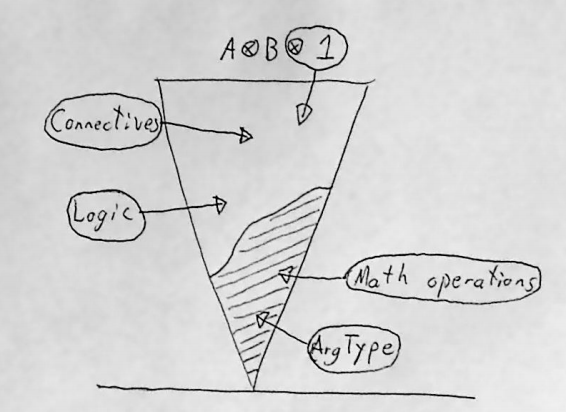
\includegraphics{Images/Picture_01}
\caption{Graphical representation of what has been translated into English and what has not.}
\label{fig:translation}
\end{figure}

This covers the important parts in the two concrete implementations, and should give the reader an idea of what the program reads and what the output will be like.